\chapter{Molybdenum disulfide (monolayer)}
In my TB model I adopted a non-orthogonal basis set of $sp_3 d_5$ orbitals considering only the nearest neighbor interactions between following pairs of atoms: $Mo - S$, $Mo-Mo$, $S-S$.
\begin{figure}[ht]
\begin{center}
\begin{subfigure}{.5\textwidth}
  \centering
  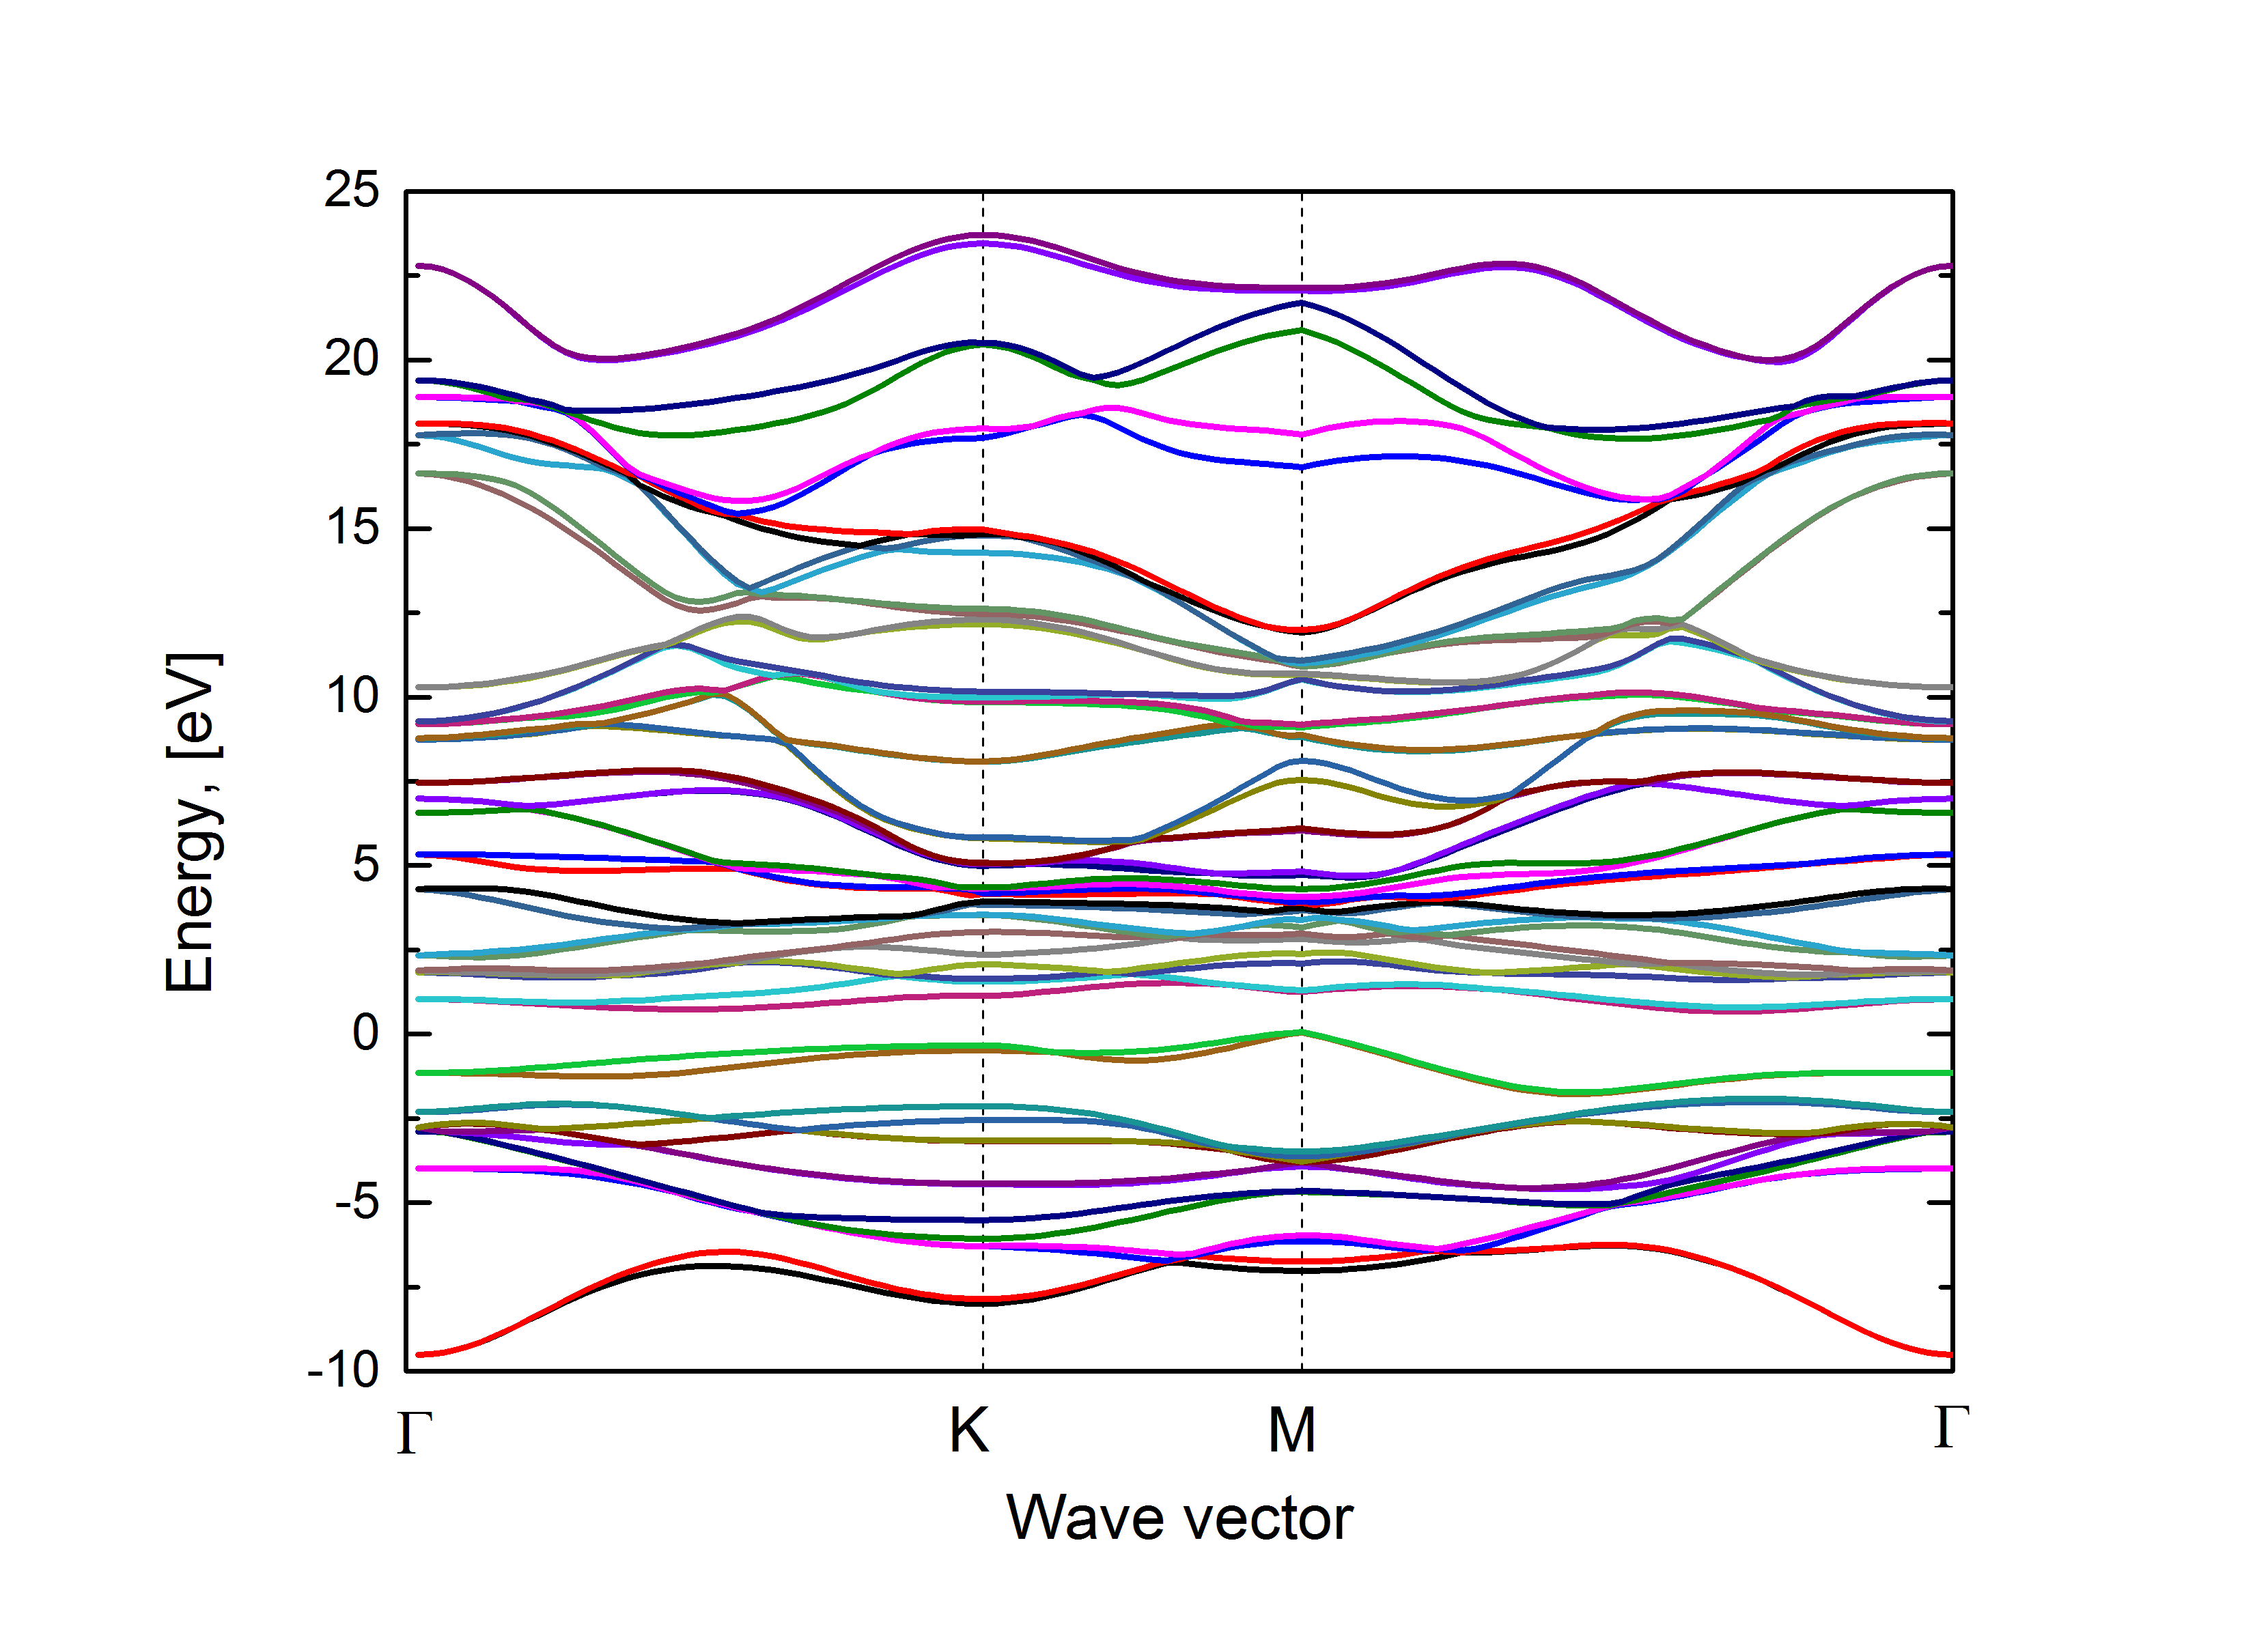
\includegraphics[width=\linewidth]{img/mos2_all}
  \label{fig:mos2_all}
\end{subfigure}%
\begin{subfigure}{.5\textwidth}
  \centering
  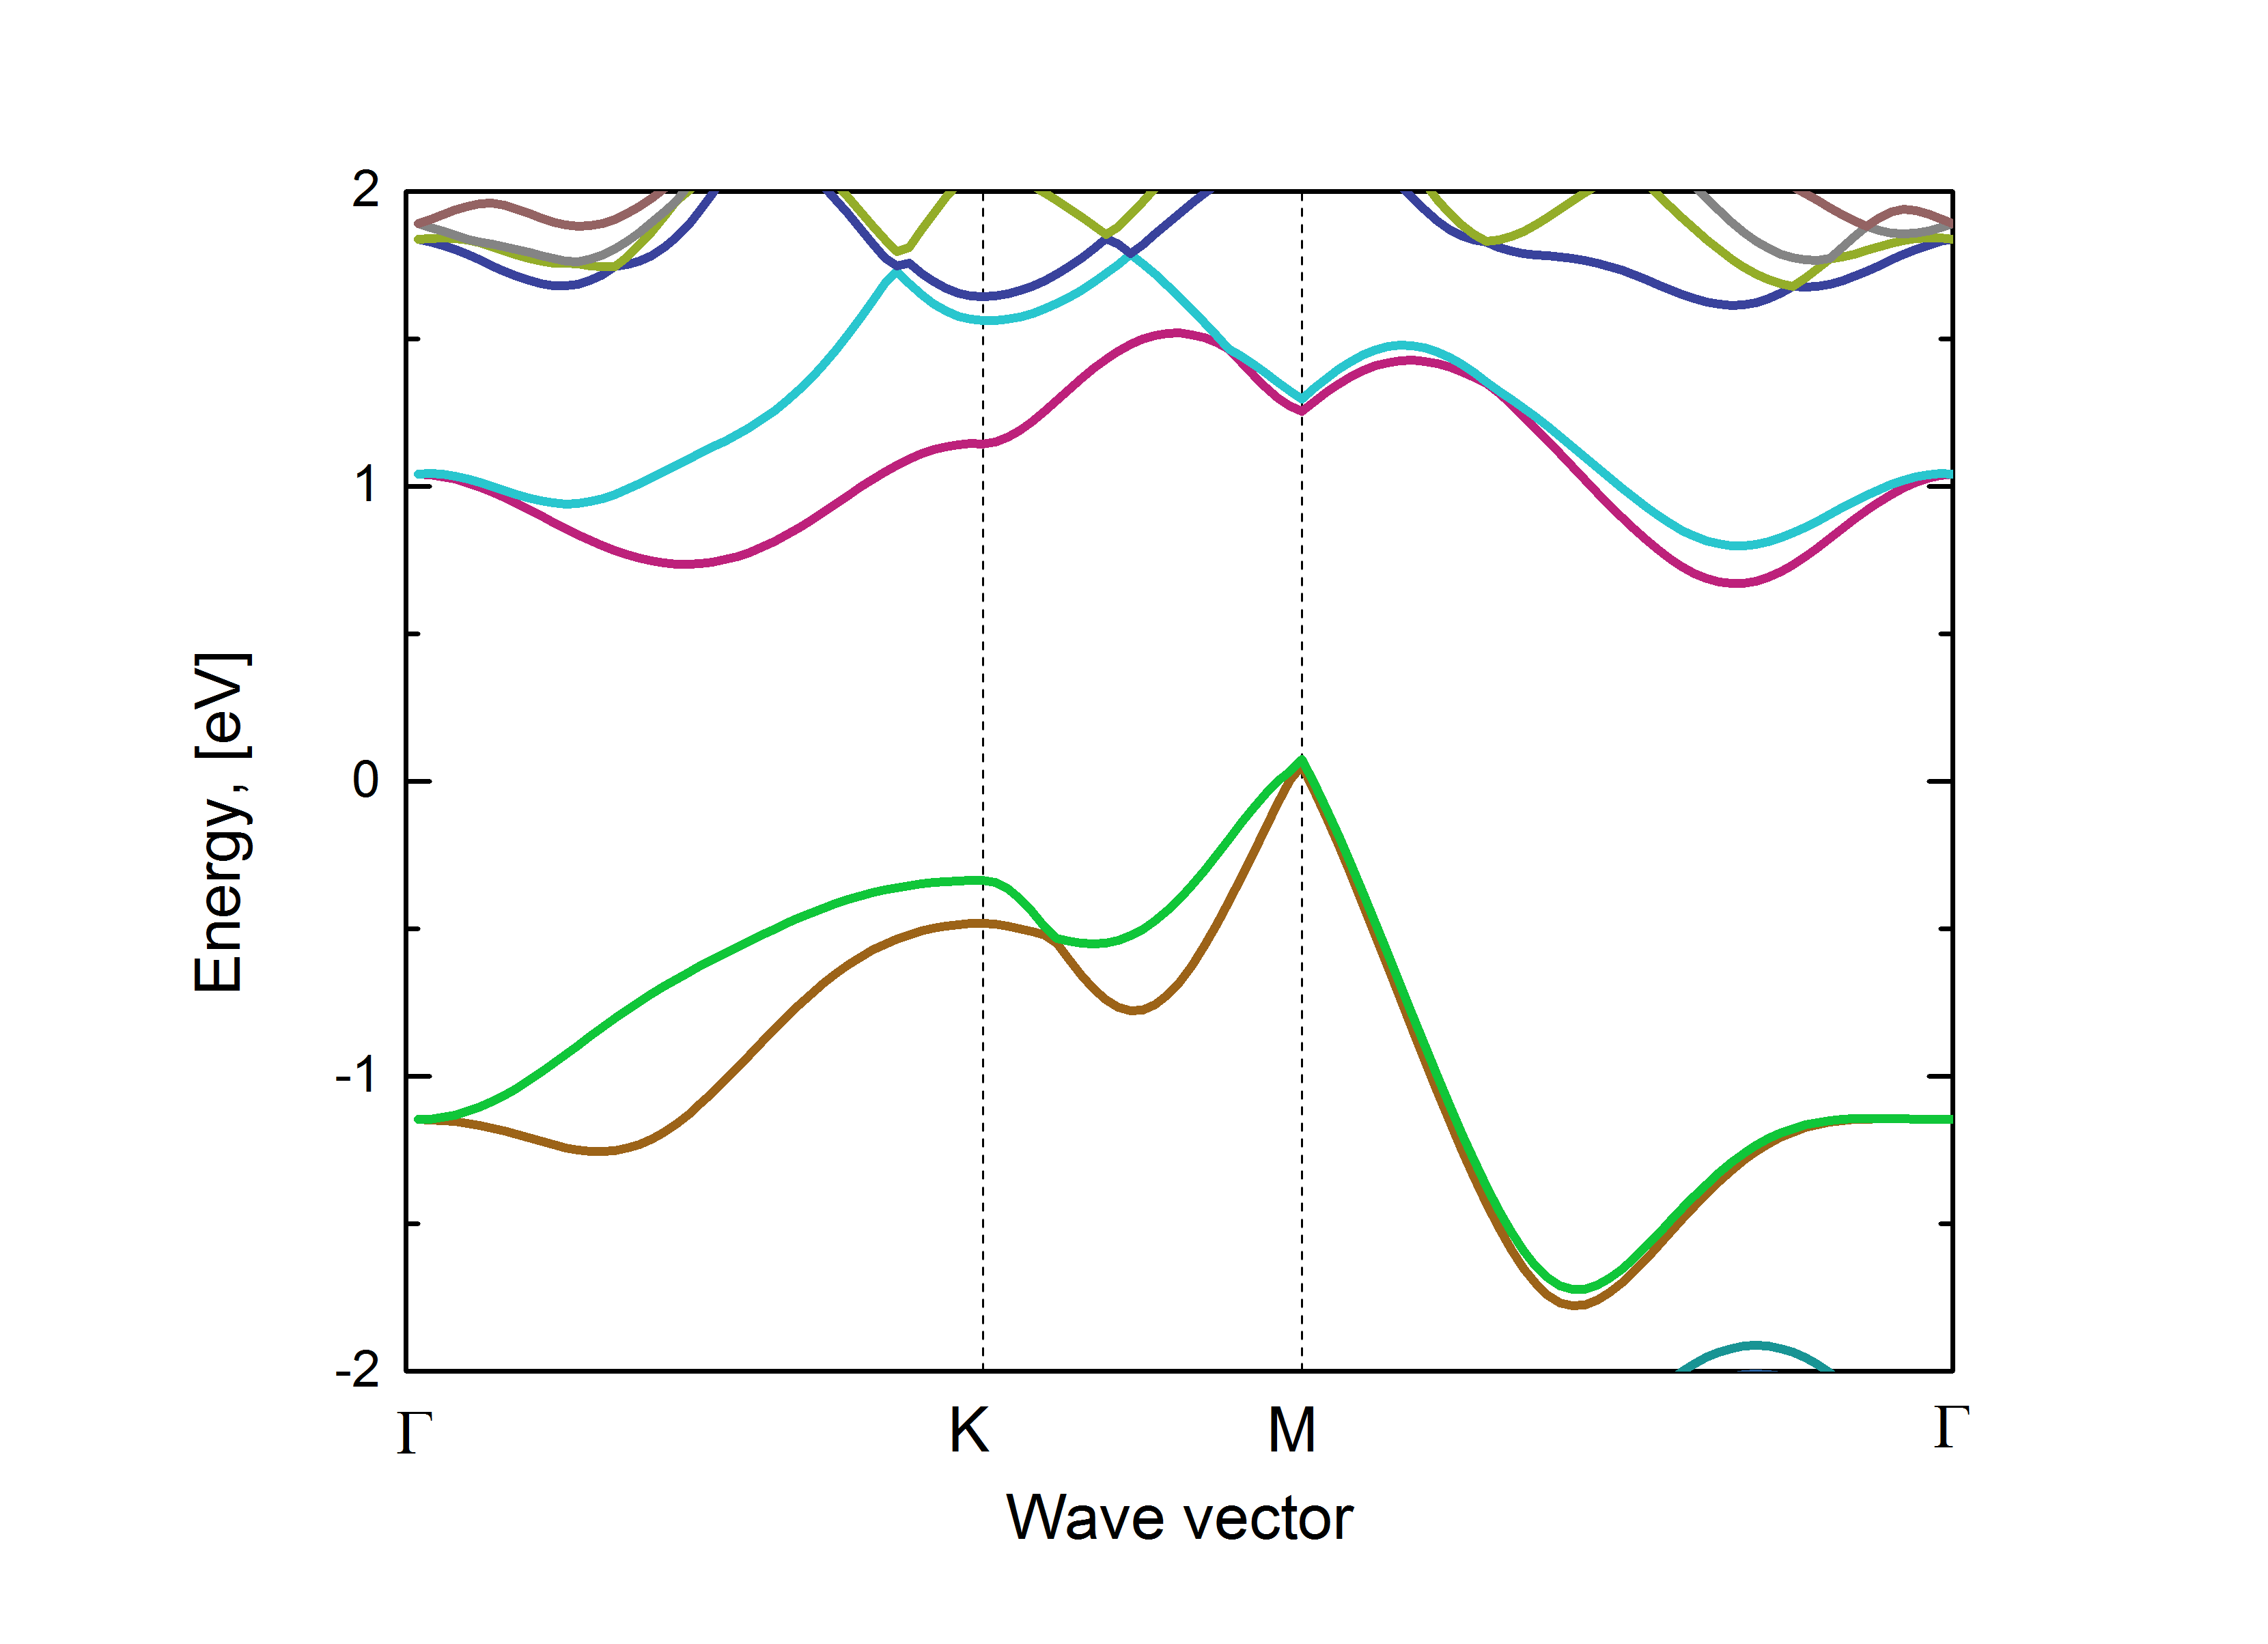
\includegraphics[width=\linewidth]{img/mos2_zoom}
  \label{fig:mos2_zoom}
\end{subfigure}
  \caption{Calculated band structure of $MoS_2$. On the right -- zoom in the surrounding of Fermi level.}
\end{center}
\end{figure}  


\begin{figure}[ht]
\begin{center}
  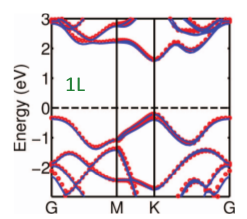
\includegraphics[width=0.3\linewidth]{img/MoS2_lit_band_struc}
  \caption{Band structure of $MoS_2$ (literature)).}
\end{center}
\end{figure}  
